\documentclass[11pt, oneside]{article} 
\usepackage{geometry}
\geometry{letterpaper} 
\usepackage{graphicx}
	
\usepackage{amssymb}
\usepackage{amsmath}
\usepackage{parskip}
\usepackage{color}
\usepackage{hyperref}

\graphicspath{{/Users/telliott/Github/calculus_book/png/}}
% \begin{center} 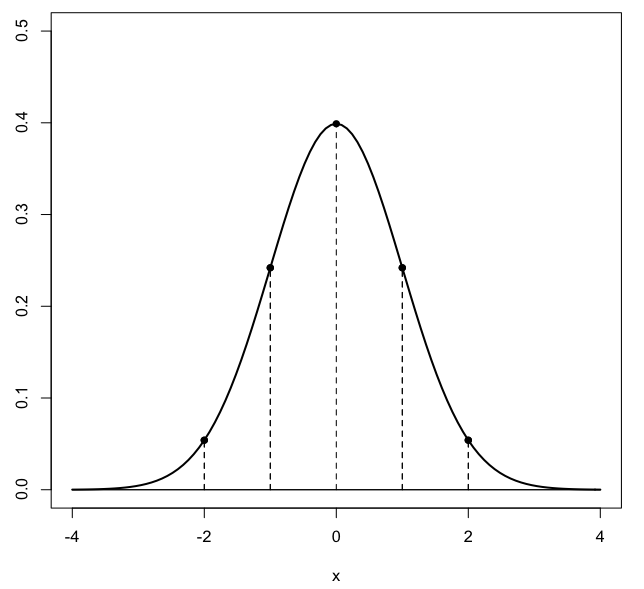
\includegraphics [scale=0.4] {gauss3.png} \end{center}

\title{Natural Numbers}
\date{}

\begin{document}
\maketitle
\Large
\section*{Integers}

The \emph{natural} or counting numbers which everyone learns very early in life are $1, 2, 3$ and so on.

One can get hung up on the question of whether the natural numbers would exist without the problem of counting three sheep or all ten of our fingers.  Leopold Kronecker said "God made the integers; all else is man's handiwork".

We will not worry about they come from.

Mathematicians refer to the \emph{set} of natural numbers and give this set a special symbol, $\mathbb{N}$.  We write
\[ \mathbb{N} = \{ 1, 2, 3 \dots \} \]

The brackets contain between them the \emph{elements} of the set. The dots mean that this sequence of numbers continue forever.

It seems hard to know how we can decide whether a particular $n$ is in the set if we can't enumerate all the members of the set.  But we can decide by its form whether $n$ is a natural number or not.  If this seems problematic, you might call $\mathbb{N}$ a class instead (Hamming);  we carry out \emph{classification} to decide whether $n$ is a natural number.

The notion of an unending sequence can be unnerving at first.

\subsection*{construction of N}

To construct the set $\mathbb{N}$, start with the smallest element, $1$.  Then add successive elements by forming $a_{n+1} = a_n + 1$.

$\mathbb{N}$ is an infinite set, meaning that there is no largest number in $\mathbb{N}$, no largest $n \in \mathbb{N}$.

Suppose $\mathbb{N}$ did have a largest number, $a$.  Well, what about $a + 1$?  By the definition we can construct it, and it is clearly also a member of the set, but $a_{n+1} > a_n$ so $a_n$ is not the largest number in the set.

$\square$

\subsection*{set membership}

The symbol $\in$ means "in the set" or "is a member of the set".

Sometimes people say that
\[ 0 \in \mathbb{N} \]
(0 is a part of the set) but most do not, and we will follow the definition given above.  If you wanted to be explicit about this you could write
\[ 0 \notin \mathbb{N} \]

What do we mean by infinity?  We mean a kind of bound on the numbers.  All numbers $n \in \mathbb{N}$ have the property that $n$ is contained in the interval $[1..\infty)$.  The right parenthesis means $\infty$ is \emph{not} part of the interval.

$\infty$ is not a number so it doesn't even make sense to write $\infty \notin \mathbb{N}$.

\subsection*{least element}

$\mathbb{N}$ does not have a greatest number, but it does have a smallest or least one.  If pairwise comparisons are carried out, a single element, the number $1$, has the property that $1 \le n$ for all numbers $n \in \mathbb{N}$.

\subsection*{well-ordered property}

Since we can also find the least member of the set excluding $1$, written $\mathbb{N} \setminus 1$, we can order every number in $\mathbb{N}$.  

This property is called the \textbf{well-ordered} property.

\subsection*{the Integers}

The set $\mathbb{Z}$ contains all the members of $\mathbb{N}$ plus their negatives, as well as the special number $0$, often called the additive identity.

\[ \mathbb{Z} = \{ \dots -2, -1, 0, 1, 2, \dots \} \]

$\mathbb{Z}$ stands for the German word \emph{Zahlen}, Number.  The set $\mathbb{Z}$ are usually referred to as the integers.

$\mathbb{Z}$ is also an infinite set and also has the well-ordered property.  To show this simply order all numbers $p > 0$ with respect to zero using $<$, and all the numbers $n < 0$ using $>$.

\subsection*{inequality}
I'm sure you've seen and used the symbols $>$ and $<$, greater than and less than.  Among the axioms of the number systems is the collection of \emph{order axioms}.  As an example:

$\circ$ \ $x < y$ means that $y - x$ is positive

$\circ$ \ $y > x$ means that $x < y$

For arbitrary numbers $a$ and $b$ one of three statements is true:  

$a < b$, $a = b$ or $a > b$.

There is no need to be systematic here.  Let us just mention that these properties (and their kin) are true not just for natural numbers, but also for the rational numbers and the real numbers, which we will talk about soon.  Here are just a few more important theorems in this class:

$\circ$ \ If $a < b$, and $c$ is any number, then $a + c < b + c$

$\circ$ \ If $a < b$, then $-b < -a$

$\circ$ \ If $a < b$ and $c > 0$, then $ac < bc$

\subsection*{algebraic operations}

$\circ$ addition:  $a + b$

$\circ$ subtraction:  $a - b = a + (-b)$

The negative integers and $0$ solve the problem of how to evaluate $a - b$ when $b \ge a$.

$\circ$ multiplication:  $a \cdot b$, also often written $ab$ (but usually not $a \times b$, at this level).

And then:

$\circ$ division $a/b$, solved by finding a number $c$ so that $c \cdot b = a$.

\subsection*{infinity is not a number}
There is a fundamental problem when we set up a division problem and $0$ is in the denominator.  What goes wrong when we attempt to divide by zero?
\[ \frac{a}{0} = \ ? \]

As we just said above, this equivalent to finding
\[ c \cdot 0 = a \]
But, by definition $c \cdot 0 = 0$.

Suppose we have $c \cdot b = a$ but not $b = 0$.  Then, as $b$ gets very small, the number $c$ can get very large.  That's OK.  We can make $c$ as large as we wish by making $b$ small enough.  But we can't say $a/0 = $ something.

If there were such a number (say $\infty$), then what about 
\[ \frac{b}{0} = \ ??  \]
\[ \frac{c}{0} = \ ??  \]

By definition, we do not allow division by zero.

And we can't answer the question what is $2 \cdot \infty$?  If we allowed multiplication by $\infty$ then the only reasonable answer would be
\[ 2 \cdot \infty = \infty \]
but then also
\[ n \cdot \infty = \infty \]
where $n$ is any number.  But then, $2 = n$.  This would be a mess.

So, by definition, \emph{infinity is not a number} and division by $0$ is \emph{undefined}.

\subsection*{limits}
Often people say that calculus is all about limits, and they are certainly a crucial part of the theoretical basis of calculus.  

We will keep the discussion of limits and $\epsilon$-$\delta$ formalism to a minimum for the reasons explained in the Introduction.  But let us try to establish an intuitive idea about what we mean when we say "in the limit as $N \rightarrow \infty$".

Above we had that there is no greatest integer.

A corollary of that is the limit
\[ \lim_{n \rightarrow \infty} \frac{(n + 1) - n}{n} = \ ?? \]
As $n$ increases without bound, the difference between successive numbers, as a fraction of $n$, tends to zero.

To get an idea about this, first simplify by multiplying by $1/n$ on top and bottom.  Then
\[ \lim_{n \rightarrow \infty} \frac{(1 + 1/n - 1)}{1} = \frac{1}{n} = 0 \]

We say that $1/n$ \emph{tends} to zero as $n$ approaches $\infty$, and so does $[(n+1)-n]/n$.

\subsection*{algebra}
As you know, the basic axioms of algebra include the following:

$\circ$ \ Commutativity for addition and multiplication: 
\[ a + b = b + a, \ \ \ a \cdot b = b \cdot a \]

$\circ$ \  Associativity for addition and multiplication:
\[ (a + b) + c = a + (b + c), \ \ \ (a \cdot b) \cdot c = a \cdot (b \cdot c) \]

$\circ$ \ Distributivity:  $a \cdot (b + c) = a \cdot b + a \cdot c$.

$\circ$ \ Additive identity:  $0 + a = a$.

$\circ$ \ Multiplicative identity:  $1 \cdot a = a$.



\end{document}